\section{Web 2.0 - Abschlussarbeiten-DB}
Im Rahmen dieses Projektes ist ein relationales Schema und eine Menge an Datens\"atzen gegeben. Ziel ist es, dieses in eine NoSQL Lösung zu übertragen und die Datens\"atze in der Datenbank zu persistieren.

\subsection{Das semantische Schema}
In der Abbildung \ref{fig:schema1} ist das Schema der Datenbank zu sehen, die in den g\"angigen NoSQL Techniken umgesetzt werden sollen. Eine Abschlussarbeit wird von einem "'Student"' oder einem "'Trainee"' geschrieben. Sowohl der "'Student"', als auch der "'Trainee"', als auch der "'Examiner"', als auch der "'Supervisor"' sind Unterklassen der Klasse "'Human"'. In Auftrag gegeben wird die Arbeit von einer "'Organisation"', die eine "'University"' oder eine "'Company"' sein kann. Die Arbeit wird eventuell von einer Menge von "'First\_Examiner"' und einer Menge von "'Second\_Examiner"' begutachtet, wenn es zu einem "'Degree"' f\"uhrt. Das mit dem "'Degree\_Topic"' verbundene "'Degree"' hat einen Titel. Das "'Topic"' kann in einer "'Topic\_Category"' liegen, in der gegebenenfalls auch der "'examiner"' oder die "'Company"' liegen. Dies bedeutet, die zentrale Klasse ist das "'Topic"', dass entweder ein "'Degree\_Topic"' oder ein "'Trainee\_Topic"' ist. Hierbei ist das "'Degree\_Topic"' wiederum entweder die "'Bachelor\_Thesis"' oder die "'Master\_Thesis"'.\\

Das Schema deutet also an, dass ein Mensch, der eine Abschlussarbeit schreibt, entweder ein Auszubildender oder ein Student ist. Diese Abschlussarbeit schreibende Person schreibt die Arbeit entweder im Rahmen einer Ausbildung oder im Rahmen eines Studiums, der mit einem Abschluss ("'Degree"') belegt ist. Fasst man dies zusammen h\"atte man eine Tabelle in der Informationen zu Abschlussarbeiten gespeichert sind. Diese enthalten neben dem "'Topic"' der Arbeit auch weitere Informationen zu den Umst\"anden. Insgesamt sind 27 Klassen gegeben, auf denen 36 Attribute verteilt sind.\\

\begin{figure}[H]
	\centering
	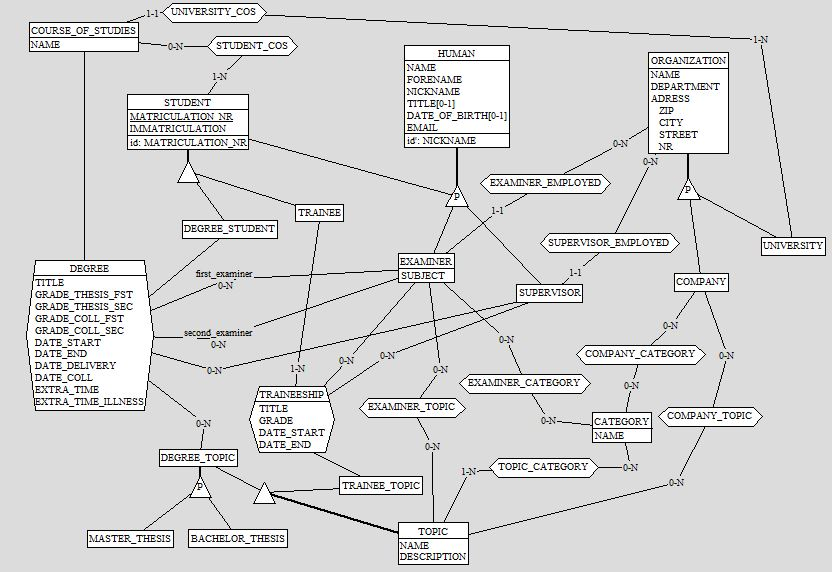
\includegraphics[scale=0.6]{images/01abschlussarbeitendbschema.jpg} 
	\caption{AbschlussarbeitenDB Schema}\label{fig:schema1}
\end{figure}

\subsection{Die Datenbestände}
Die Tats\"achlichen Daten unterscheiden sich stark von den in dem Schema \ref{fig:schema1} dargestellten Sachverhalten. Wie in Abbildung \ref{fig:schema2} zu sehen gibt es insgesamt 21 Spalten. Insgesamt umfasst die Datenbasis 1637 Datensätze. \\

\begin{figure}[H]
	\centering
	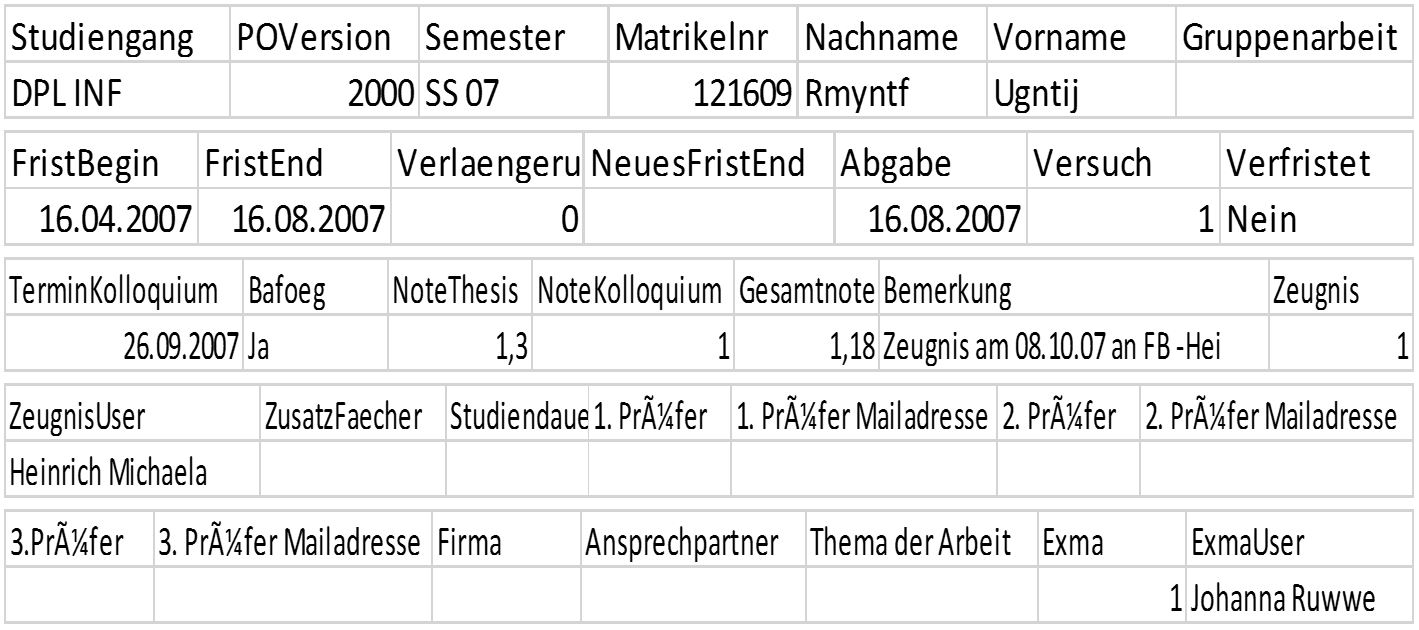
\includegraphics[scale=0.3]{images/01beispieldatensatzcsv.jpg} 
	\caption{Beispiel-Datensatz}\label{fig:schema2}
\end{figure}

Im Vergleich mit dem Schema f\"allt auf, dass es scheinbar einige Probleme gibt. Die erhobenen Daten weisen folgende Probleme auf:\\
\begin{itemize}
\item Die 21 Spalten repr\"asentieren 21 Attribute, die eine deutliche Differenz zu den 36 Attributen des Schemas darstellen. Dies bedeutet, in den Datenbest\"anden sind weniger Informationen gegeben, als eigentlich im Schema festgelegt.
\item In den Daten kommen Attribute vor, die im Schema nicht erw\"ahnt wurden. Dies umfasst Attribute wie z.B. "'Gruppenarbeit"' oder "'Bafoeg"'.
\item Einige Attribute verfügen über andere Bezeichnungen, als in dem Schema genannt werden. So hat ein Student laut Schema eine "'Matriculation\_NR"'. In den Daten ist dieses Attribut jedoch unter der Bezeichnung "'Matrikelnr"' aufgef\"uhrt.
\item In den Spalten der Daten sind einige Attribute mit Sonderzeichen belegt, was bei der \"Ubertragung der Daten in eine NoSQL Datenbank zu Problemen führen kann.
\item Einige Spalten enthalten keine Werte, was bei der \"Ubertragung der Daten in die Datenbank gegebenenfalls ber\"ucksichtigt werden muss. Besonders kritisch ist dies in den F\"allen zu sehen, bei denen das "'Thema der Arbeit"' keinen Wert hat.
\item Ein Problem der Daten ist, dass ein Professor teilweise unter verschiedenen Bezeichnungen in der Tabelle aufgeführt ist. \\
\end{itemize}

Bei der \"Ubertragung der Daten in eine Datenbank, müssen L\"osungen für die verschiedenen Probleme gefunden werden. Hier muss vor allem entschieden werden, welches Objekt bei der Migration in die NoSQL Datenbank wichtiger ist. Wird dem Schema gr\"o\ss{}ere Beachtung geschenkt, m\"ussen gr\"o\ss{}ere Anpassungen an den Daten vorgenommen werden. Sollten die Daten gr\"o\ss{}ere Priorit\"at haben, muss die Rolle des Schemas und dessen G\"ultigkeit \"uberdacht werden.\\
